
Bending machine as a unit comes with a terminal and a foot pedal. Terminal is used to operate
the bending machine for starting, stopping and configuring the bending machine and also loading the bending program.
Foot pedal comes with two pedals, one for closing the bending machine and other for opening of the bending machine.
Opening and closing of bending machine is controlled by a foot pedal for the manual bending operations.

\begin{figure}[h]
    \centering
    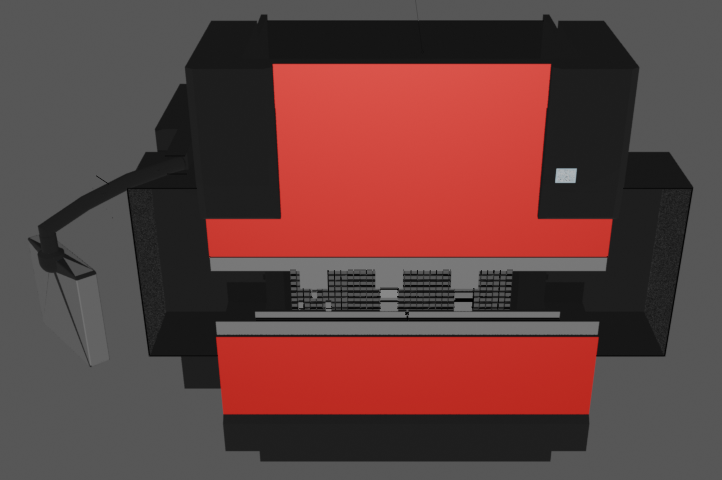
\includegraphics[width=0.75\textwidth]{figures/bending-machine-blender.png}
    \caption{Bending machine asset in simulation}
    \label{fig:bending-machine-blender}
\end{figure}
To automate the bending machine, \hyperref[acro:PLC]{PLC} is used to send signals to foot pedal which in turn, controls the opening and closing of bending machine.

An inspection camera is also added to measure the bending angle after each bending operation. This inspection camera is operated by the PLC
and the bending angles are saved in \textit{.csv} file format and displayed on an \hyperref[acro:HMI]{HMI}.
